%% LyX 2.1.4 created this file.  For more info, see http://www.lyx.org/.
%% Do not edit unless you really know what you are doing.
\documentclass[ruled]{article}
\usepackage{courier}
\usepackage[latin9]{inputenc}
\usepackage[letterpaper]{geometry}
\geometry{verbose}
\usepackage{url}
\usepackage{algorithm2e}
\usepackage{amsmath}
\usepackage{graphicx}
\usepackage[unicode=true,
 bookmarks=false,
 breaklinks=false,pdfborder={0 0 1},backref=section,colorlinks=false]
 {hyperref}

\makeatletter

%%%%%%%%%%%%%%%%%%%%%%%%%%%%%% LyX specific LaTeX commands.
\providecommand{\LyX}{\texorpdfstring%
  {L\kern-.1667em\lower.25em\hbox{Y}\kern-.125emX\@}
  {LyX}}
%% Special footnote code from the package 'stblftnt.sty'
%% Author: Robin Fairbairns -- Last revised Dec 13 1996
\let\SF@@footnote\footnote
\def\footnote{\ifx\protect\@typeset@protect
    \expandafter\SF@@footnote
  \else
    \expandafter\SF@gobble@opt
  \fi
}
\expandafter\def\csname SF@gobble@opt \endcsname{\@ifnextchar[%]
  \SF@gobble@twobracket
  \@gobble
}
\edef\SF@gobble@opt{\noexpand\protect
  \expandafter\noexpand\csname SF@gobble@opt \endcsname}
\def\SF@gobble@twobracket[#1]#2{}

%%%%%%%%%%%%%%%%%%%%%%%%%%%%%% User specified LaTeX commands.
\title{DS-GA 1003: Machine Learning and Computational Statistics\\
Homework 5: Trees and Boosting} 
\date{} 

\usepackage{amsfonts}\usepackage{capt-of}
%\usepackage{url}
\usepackage{graphicx}
\usepackage{color}
\usepackage{bbm}
\usepackage{enumerate}
\newcommand{\carlos}[1]{\textcolor{red}{Carlos: #1}}
\newcommand{\field}[1]{\mathbb{#1}} 
\newcommand{\hide}[1]{#1}
\newcommand{\pd}[2]{\frac{\partial #1}{\partial #2}}
\providecommand{\m}[1]{\mathbf{#1}}
\providecommand{\norm}[1]{\left\|#1\right\|}
\providecommand{\sign}[1]{\text{sign}\left(#1\right)}
\DeclareMathOperator*{\argmin}{arg\,min}
\providecommand{\what}{\m{\hat{w}}}
\providecommand{\dw}{\Delta w}
\providecommand{\dmw}{\Delta \m{w}}
\providecommand{\hy}{\hat{y}}

\makeatother

\begin{document}
\global\long\def\reals{\mathbf{R}}
 \global\long\def\integers{\mathbf{Z}}
\global\long\def\naturals{\mathbf{N}}
 \global\long\def\rationals{\mathbf{Q}}
\global\long\def\ca{\mathcal{A}}
\global\long\def\cb{\mathcal{B}}
 \global\long\def\cc{\mathcal{C}}
 \global\long\def\cd{\mathcal{D}}
\global\long\def\ce{\mathcal{E}}
\global\long\def\cf{\mathcal{F}}
\global\long\def\cg{\mathcal{G}}
\global\long\def\ch{\mathcal{H}}
\global\long\def\ci{\mathcal{I}}
\global\long\def\cj{\mathcal{J}}
\global\long\def\ck{\mathcal{K}}
\global\long\def\cl{\mathcal{L}}
\global\long\def\cm{\mathcal{M}}
\global\long\def\cn{\mathcal{N}}
\global\long\def\co{\mathcal{O}}
\global\long\def\cp{\mathcal{P}}
\global\long\def\cq{\mathcal{Q}}
\global\long\def\calr{\mathcal{R}}
\global\long\def\cs{\mathcal{S}}
\global\long\def\ct{\mathcal{T}}
\global\long\def\cu{\mathcal{U}}
\global\long\def\cv{\mathcal{V}}
\global\long\def\cw{\mathcal{W}}
\global\long\def\cx{\mathcal{X}}
\global\long\def\cy{\mathcal{Y}}
\global\long\def\cz{\mathcal{Z}}
\global\long\def\ind#1{1(#1)}
\global\long\def\pr{\mathbb{P}}
\global\long\def\predsp{\cy}
\global\long\def\outsp{\cy}
\global\long\def\prxy{P_{\cx\times\cy}}
\global\long\def\prx{P_{\cx}}
\global\long\def\prygivenx{P_{\cy\mid\cx}}
\global\long\def\ex{\mathbb{E}}
\global\long\def\var{\textrm{Var}}
\global\long\def\cov{\textrm{Cov}}
\global\long\def\sgn{\textrm{sgn}}
\global\long\def\sign{\textrm{sign}}
\global\long\def\kl{\textrm{KL}}
\global\long\def\law{\mathcal{L}}
\global\long\def\eps{\varepsilon}
\global\long\def\as{\textrm{ a.s.}}
\global\long\def\io{\textrm{ i.o.}}
\global\long\def\ev{\textrm{ ev.}}
\global\long\def\convd{\stackrel{d}{\to}}
\global\long\def\eqd{\stackrel{d}{=}}
\global\long\def\del{\nabla}
\global\long\def\loss{\ell}
\global\long\def\risk{R}
\global\long\def\emprisk{\hat{R}_{\ell}}
\global\long\def\lossfnl{L}
\global\long\def\emplossfnl{\hat{L}}
\global\long\def\empminimizer#1{\hat{#1}_{\ell}}
\global\long\def\minimizer#1{#1_{*}}
\global\long\def\etal{\textrm{et. al.}}
\global\long\def\tr{\operatorname{tr}}
\global\long\def\trace{\operatorname{trace}}
\global\long\def\diag{\text{diag}}
\global\long\def\rank{\text{rank}}
\global\long\def\linspan{\text{span}}
\global\long\def\proj{\text{Proj}}
\global\long\def\argmax{\operatornamewithlimits{arg\, max}}
\global\long\def\argmin{\operatornamewithlimits{arg\, min}}
\global\long\def\bfx{\mathbf{x}}
\global\long\def\bfy{\mathbf{y}}
\global\long\def\bfl{\mathbf{\lambda}}
\global\long\def\bfm{\mathbf{\mu}}
\global\long\def\calL{\mathcal{L}}
\global\long\def\vw{\boldsymbol{w}}
\global\long\def\vx{\boldsymbol{x}}
\global\long\def\vxi{\boldsymbol{\xi}}
\global\long\def\valpha{\boldsymbol{\alpha}}
\global\long\def\vbeta{\boldsymbol{\beta}}
\global\long\def\vsigma{\boldsymbol{\sigma}}
\global\long\def\vmu{\boldsymbol{\mu}}
\global\long\def\vtheta{\boldsymbol{\theta}}
\global\long\def\vd{\boldsymbol{d}}
\global\long\def\vs{\boldsymbol{s}}
\global\long\def\vt{\boldsymbol{t}}
\global\long\def\vh{\boldsymbol{h}}
\global\long\def\ve{\boldsymbol{e}}
\global\long\def\vf{\boldsymbol{f}}
\global\long\def\vg{\boldsymbol{g}}
\global\long\def\vz{\boldsymbol{z}}
\global\long\def\vk{\boldsymbol{k}}
\global\long\def\va{\boldsymbol{a}}
\global\long\def\vb{\boldsymbol{b}}
\global\long\def\vv{\boldsymbol{v}}
\global\long\def\vy{\boldsymbol{y}}
\global\long\def\hil{\ch}
\global\long\def\rkhs{\hil}
\maketitle

\textbf{Due: Monday, April 4, 2016, at 6pm (Submit via NYU Classes)}

\textbf{Instructions}: Your answers to the questions below, including
plots and mathematical work, should be submitted as a single file,
either HTML or PDF. You may include your code inline or submit it
as a separate file. You may either scan hand-written work or, preferably,
write your answers using software that typesets mathematics (e.g.
\LaTeX, \LyX{}, or MathJax via iPython).


\section{Dataset description}

You will be working with a simple two-feature binary dataset, known
as the Banana dataset\footnote{\url{http://mldata.org/repository/data/viewslug/banana-ida/}},
which can be visualized as follows:

\begin{center}
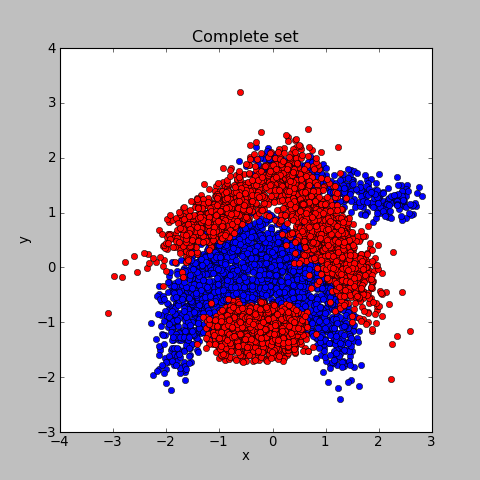
\includegraphics[width=0.4\textwidth]{banana}\\
 (Source: \url{http://adessowiki.fee.unicamp.br/adesso/wiki/courseIA368Q1S2012/eri_test_2/view/}) 
\par\end{center}

The data consists of 5,300 instances, which have been split into 3,500
training points and 1,800 test points for this assignment. The csv
files are included in the \texttt{data} directory. Each row corresponds
to a data point - the first entry of the row gives the class label,
and the next two entries give the values of the attributes.


\section{Decision Trees }


\subsection{\label{sub:Trees-on-the-banana-dataset}Trees on the Banana Dataset}

The official \texttt{sklearn} documentation provides code that constructs
a decision tree and visualizes the decision boundary on the ``Iris\footnote{\url{https://archive.ics.uci.edu/ml/datasets/Iris}}
dataset'' (\url{http://scikit-learn.org/stable/auto_examples/tree/plot_iris.html#example-tree-plot-iris-py}).
Note that the \texttt{sklearn} implementation of decision trees is
a bit different from that described in lecture: they just build to
a certain depth, without a pruning step. 
\begin{enumerate}
\item Modify the code referenced above to work on the Banana dataset. The
default class labels are -1 and 1 in the given data files, but for
the visualization code snippet to work, you will have to modify the
class labels to 0 and 1. Note that the Iris dataset is a multiclass
problem with 3 classes, while the Banana dataset is a binary dataset. 
\item Run your code for different depths of decision trees, from 1 through
10, and briefly describe your observations of the decision surface
visualization. {[}Use the default values for all other parameters.{]} 
\item Plot the train and test errors as a function of the depth. Again,
give a brief description of your observations. 
\item {[}Optional{]} Experiment with the other hyperparameters provided
by \texttt{DecisionTreeClassifier} and find the combination giving
the smallest test error. Summarize what you learn. 
\end{enumerate}

\section{AdaBoost}


\subsection{Implementation}

In this problem, you will implement AdaBoost, one of the most popular
techniques in ensemble methods. 
\begin{enumerate}
\item Implement AdaBoost for the Banana dataset with decision trees of depth
3 as the weak classifiers (also known as ``base classifiers'').
Use the decision tree implementation from \texttt{sklearn} as in \ref{sub:Trees-on-the-banana-dataset}.
The \texttt{fit} function of \texttt{DecisionTreeClassifier} has a
parameter \texttt{sample\_weight,} which you can use to weigh training
examples differently during various rounds of AdaBoost. 
\item {[}Optional{]} Visualize the AdaBoost training procedure for different
numbers of rounds from 1 through 10. Plot the decision surface, and
the training examples, such that training samples with larger weights
in any round are represented as larger points compared to those with
smaller weights. Provide a brief description of your observations. 
\item Plot the train and test errors as a function of the number of rounds
from 1 through 10. Again, give a brief description of your observations. 
\end{enumerate}

\section{Gradient Boosting Machines}

Recall the general gradient boosting algorithm\footnote{Besides the lecture slides, you can find an accessible discussion
of this approach in \url{http://www.saedsayad.com/docs/gbm2.pdf},
in one of the original references \url{http://statweb.stanford.edu/~jhf/ftp/trebst.pdf},
and in this review paper \url{http://web.stanford.edu/~hastie/Papers/buehlmann.pdf}. }, for a given loss function $\ell$ and a hypothesis space $\cf$
of regression functions (i.e. functions mapping from the input space
to $\reals$): 
\begin{enumerate}
\item Initialize $f_{0}(x)=0$. 
\item For $m=1$ to $M$:

\begin{enumerate}
\item Compute: 
\[
{\bf g}_{m}=\left(\left.\frac{\partial}{\partial f(x_{i})}\sum_{i=1}^{n}\ell\left(y_{i},f(x_{i})\right)\right|_{f(x_{i})=f_{m-1}(x_{i})}\right)_{i=1}^{n}
\]

\item Fit regression model to $-{\bf g}_{m}$: 
\[
h_{m}=\argmin_{h\in\cf}\sum_{i=1}^{n}\left(\left(-{\bf g}_{m}\right)_{i}-h(x_{i})\right)^{2}.
\]

\item Choose fixed step size $\nu_{m}=\nu\in(0,1]$, or take 
\[
\nu_{m}=\argmin_{\nu>0}\sum_{i=1}^{n}\ell\left(y_{i},f_{m-1}(x_{i})+\nu h_{m}(x_{i})\right).
\]

\item Take the step: 
\[
f_{m}(x)=f_{m-1}(x)+\nu_{m}h_{m}(x)
\]

\end{enumerate}
\item Return $f_{M}$. 
\end{enumerate}
In this problem we'll derive two special cases of the general gradient
boosting framework: $L_{2}$-Boosting and BinomialBoost. 
\begin{enumerate}
\item Consider the regression framework, where $\cy=\reals$. Suppose our
loss function is given by 
\[
\ell(\hat{y},y)=\frac{1}{2}\left(\hat{y}-y\right)^{2},
\]
and at the beginning of the $m$'th round of gradient boosting, we
have the function $f_{m-1}(x)$. Show that the $h_{m}$ chosen as
the next basis function is given by 
\[
h_{m}=\argmin_{h\in\cf}\sum_{i=1}^{n}\left[\left(y_{i}-f_{m-1}(x_{i})\right)-h(x_{i})\right]^{2}.
\]
In other words, at each stage we find the weak prediction function
$h_{m}\in\cf$ that is the best fit to the residuals from the previous
stage. {[}Hint: Once you understand what's going on, this is a pretty
easy problem.{]} 
\item Now let's consider the classification framework, where $\cy=\left\{ -1,1\right\} $.
In lecture, we noted that AdaBoost corresponds to forward stagewise
additive modeling with the exponential loss, and that the exponential
loss not very robust to outliers (i.e. outliers can have a large effect
on the final prediction function). Instead, let's consider instead
the logistic loss 
\[
\ell(m)=\ln\left(1+e^{-m}\right),
\]
where $m=yf(x)$ is the margin. Similar to what we did in the $L_{2}$-Boosting
question, write an expression for $h_{m}$ as an argmin over $\cf$. 
\end{enumerate}

\section{From Margins to Conditional Probabilities\protect\footnote{This problem is based on Section 7.5.3 of Schapire and Freund's book
\emph{Boosting: Foundations and Algorithms}.}}

Let's consider the classification setting, in which $\left(x_{1},y_{1}\right),\ldots,\left(x_{n},y_{n}\right)\in\cx\times\left\{ -1,1\right\} $
are sampled i.i.d. from some unknown distribution. For a prediction
function $f:\cx\to\reals$, we define the \textbf{margin }on an example
$\left(x,y\right)$ to be $m=yf(x)$. Since our class predictions
are given by $\sign(f(x))$, we see that a prediction is correct iff
$m(x)>0$. We have said we can interpret the magnitude of the margin
$\left|m(x)\right|$ as a measure of confidence. However, it is not
clear what the ``units'' of the margin are, so it is hard to interpret
the magnitudes beyond saying one prediction is more or less confident
than another. In this problem, we investigate how we can translate
the margin into a conditional probability, which is much easier to
interpret. In other words, we are looking for a mapping $m(x)\mapsto p(y=1\mid x)$. 

In this problem we will consider margin losses. A loss function is
a \textbf{margin loss} if it can be written in terms of the margin
$m=yf(x)$. We are interested in how we can go from an empirical risk
minimizer of a margin loss, $\hat{f}=\argmin_{f\in\cf}\sum_{i=1}^{n}\ell\left(y_{i}f(x_{i})\right)$,
to a conditional probability estimator $\hat{\pi}(x)\approx p(y=1\mid x)$.
Our approach will be to find the mapping in terms of the Bayes prediction
function\footnote{In this context, the Bayes prediction function is often referred to
as the ``population minimizer.'' The term ``population'' makes
most sense in a context where we are using a sample to approximate
some statistic of an entire population. In our case, ``population''
referes to the fact that we are minimizing with respect to the true
distribution, rather than a sample.}, and then apply the same mapping to the empirical risk minimizer.
While there is plenty that can go wrong with this ``plug-in'' approach
(primarily, the empirical risk minimizer from a hypothesis space $\cf$
may be a poor estimate for the Bayes prediction function), it is at
least well-motivated, and it can work well in practice. And please
note that we can do better than just hoping for success: if you have
enough validation data, you can directly assess how well ``calibrated''
the predicted probabilities are. This blog post has some discussion
of calibration plots: \href{https://jmetzen.github.io/2015-04-14/calibration.html}{https://jmetzen.github.io/2015-04-14/calibration.html}. 

It turns out it is straightforward to find the Bayes prediction function
$f^{*}$ for margin losses, at least in terms of the data-generating
distribution: For any given $x\in\cx$, we'll find the best possible
prediction $\hat{y}$. This will be the $\hat{y}$ that minimizes
\[
\ex_{y}\left[\ell\left(y\hat{y}\right)\mid x\right].
\]
If we can calculate this $\hat{y}$ for all $x\in\cx$, then we will
have determined $f^{*}(x)$. We will simply take
\[
f^{*}(x)=\argmin_{\hat{y}}\ex_{y}\left[\ell\left(y\hat{y}\right)\mid x\right].
\]
It may be intuitively obvious that this $f^{*}$ is the risk minimizer.
Here's a mathematical proof: 
\begin{eqnarray*}
\min_{f}\ex_{x,y}\ell\left(yf(x)\right) & = & \min_{f}\ex_{x}\left[\ex_{y}\left[\ell\left(yf(x)\right)\mid x\right]\right]\\
 & \ge & \ex_{x}\left[\min_{\hat{y}}\ex_{y}\left[\ell\left(y\hat{y}\right)\mid x\right]\right]\\
 & = & \ex_{x}\left[\ex_{y}\left[\ell\left(yf^{*}(x)\right)\mid x\right]\right]\\
 & = & \ex_{x,y}\ell\left(yf^{*}(x)\right).
\end{eqnarray*}
But of course we must also have $\min_{f}\ex_{x,y}\ell\left(yf(x)\right)\le\ex_{x,y}\ell\left(yf^{*}(x)\right)$.
So the inequality must actually be an equality, and thus the minimum
is attained at $f^{*}$.

Below we'll calculate $f^{*}$ for several loss functions. It will
be convenient to let $\pi(x)=\pr\left(y=1\mid x\right)$ in the work
below.
\begin{enumerate}
\item Write $\ex_{y}\left[\ell\left(yf(x)\right)\mid x\right]$ in terms
of $\pi(x)$ and $\ell\left(f(x)\right)$. {[}Hint: Use the fact that
$y\in\left\{ -1,1\right\} $.{]}
\item Show that the Bayes prediction function $f^{*}(x)$ for the exponential
loss function $\ell\left(y,f(x)\right)=e^{-yf(x)}$ is given by 
\[
f^{*}(x)=\frac{1}{2}\ln\left(\frac{\pi(x)}{1-\pi(x)}\right)
\]
and, given the Bayes prediction function $f^{*}$, we can recover
the conditional probabilities by
\[
\pi(x)=\frac{1}{1+e^{-2f^{*}(x)}}.
\]
{[}Hint: Differentiate the expression in the previous problem with
respect to $f(x)$. If this is confusing, you may find it more comforting
to change variables a bit: Fix an $x\in\cx$. Then write $p=\pi(x)$
and $\hat{y}=f(x)$. After substituting these into the expression
you had for the previous problem, you'll want to find $\hat{y}$ that
minimizes the expression. Use differential calculus. Once you've done
it for a single $x$, it's easy to write the solution as a function
of $x$.{]} 
\item Show that the Bayes prediction function $f^{*}(x)$ for the logistic
loss function $\ell\left(y,f(x)\right)=\ln\left(1+e^{-yf(x)}\right)$
is given by
\[
f^{*}(x)=\ln\left(\frac{\pi(x)}{1-\pi(x)}\right)
\]
and the conditional probabilities are given by
\[
\pi(x)=\frac{1}{1+e^{-f^{*}(x)}}.
\]
 Again, we may assume that $\pi(x)\in(0,1)$.
\item {[}Optional{]} Show that the Bayes prediction function $f^{*}(x)$
for the hinge loss function $\ell\left(y,f(x)\right)=\max\left(0,1-yf(x)\right)$
is given by
\[
f^{*}(x)=\sign\left(\pi(x)-\frac{1}{2}\right).
\]
Note that it is impossible to recover $\pi(x)$ from $f^{*}(x)$ in
this scenario. However, in practice we work with an empirical risk
minimizer, from which we may still be able to recover a reasonable
estimate for $\pi(x)$. An early approach to this problem is known
as ``Platt scaling'': \href{https://en.wikipedia.org/wiki/Platt_scaling}{https://en.wikipedia.org/wiki/Platt\_{}scaling}. \end{enumerate}

\end{document}
